% Point spreads for two runs of blah

\begin{figure}
\center

% TODO: actual images

\begin{subfigure}[b]{0.45\textwidth}
	%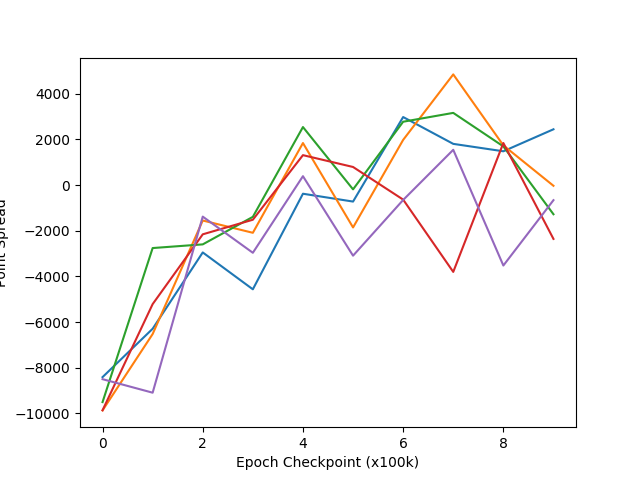
\includegraphics[width=\linewidth]{images/findings/experiments/learning_rate/tourny_a.png}
	\caption{A trained agent plays against previous iterations of itself.}
	\label{fig:expts-sanitycheck-spreads-a}
\end{subfigure}
~
\begin{subfigure}[b]{0.45\textwidth}
	%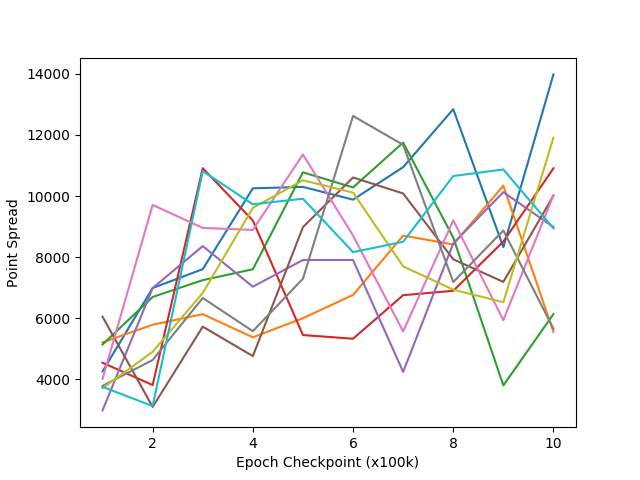
\includegraphics[width=\linewidth]{images/findings/experiments/learning_rate/tourny_b.png}
	\caption{
		An agent using a semi-pure \handmaxavg\ strategy
		plays the epoch checkpoints of an agent which has been trained
		against this strategy.
	}
	\label{fig:expts-sanitycheck-spreads-b}
\end{subfigure}

\caption{
	Point spreads of several 10,000-game tournaments between agents of varying
	training levels when started with set of semi-pure \handmaxavg\ strategy
	weights.
}
\label{fig:expts-sanitycheck-spreads}
\end{figure}
